%!TEX root = ../../main.tex

\section{Methods}	\label{sec::methods}

	\begin{figure}[tp]
		\begin{subfigure}[t]{ 0.49\linewidth}
			\centering
			\testbox{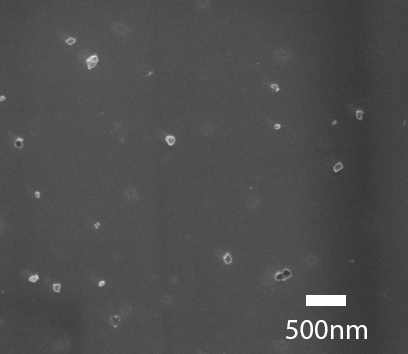
\includegraphics[trim = 0 0 0 0,  clip= true, height=5cm]{./pics/Ir27M_mitte_213_151111_22_crop.jpg}}
			\caption{}\label{subfig::sem}
			% \caption{SEM picture of the milled nanodiamonds of a mean diameter of \SI{100}{\nano\meter}}
		\end{subfigure}
		\hfill
		\begin{subfigure}[t]{ 0.49\linewidth}
			\centering
			\testbox{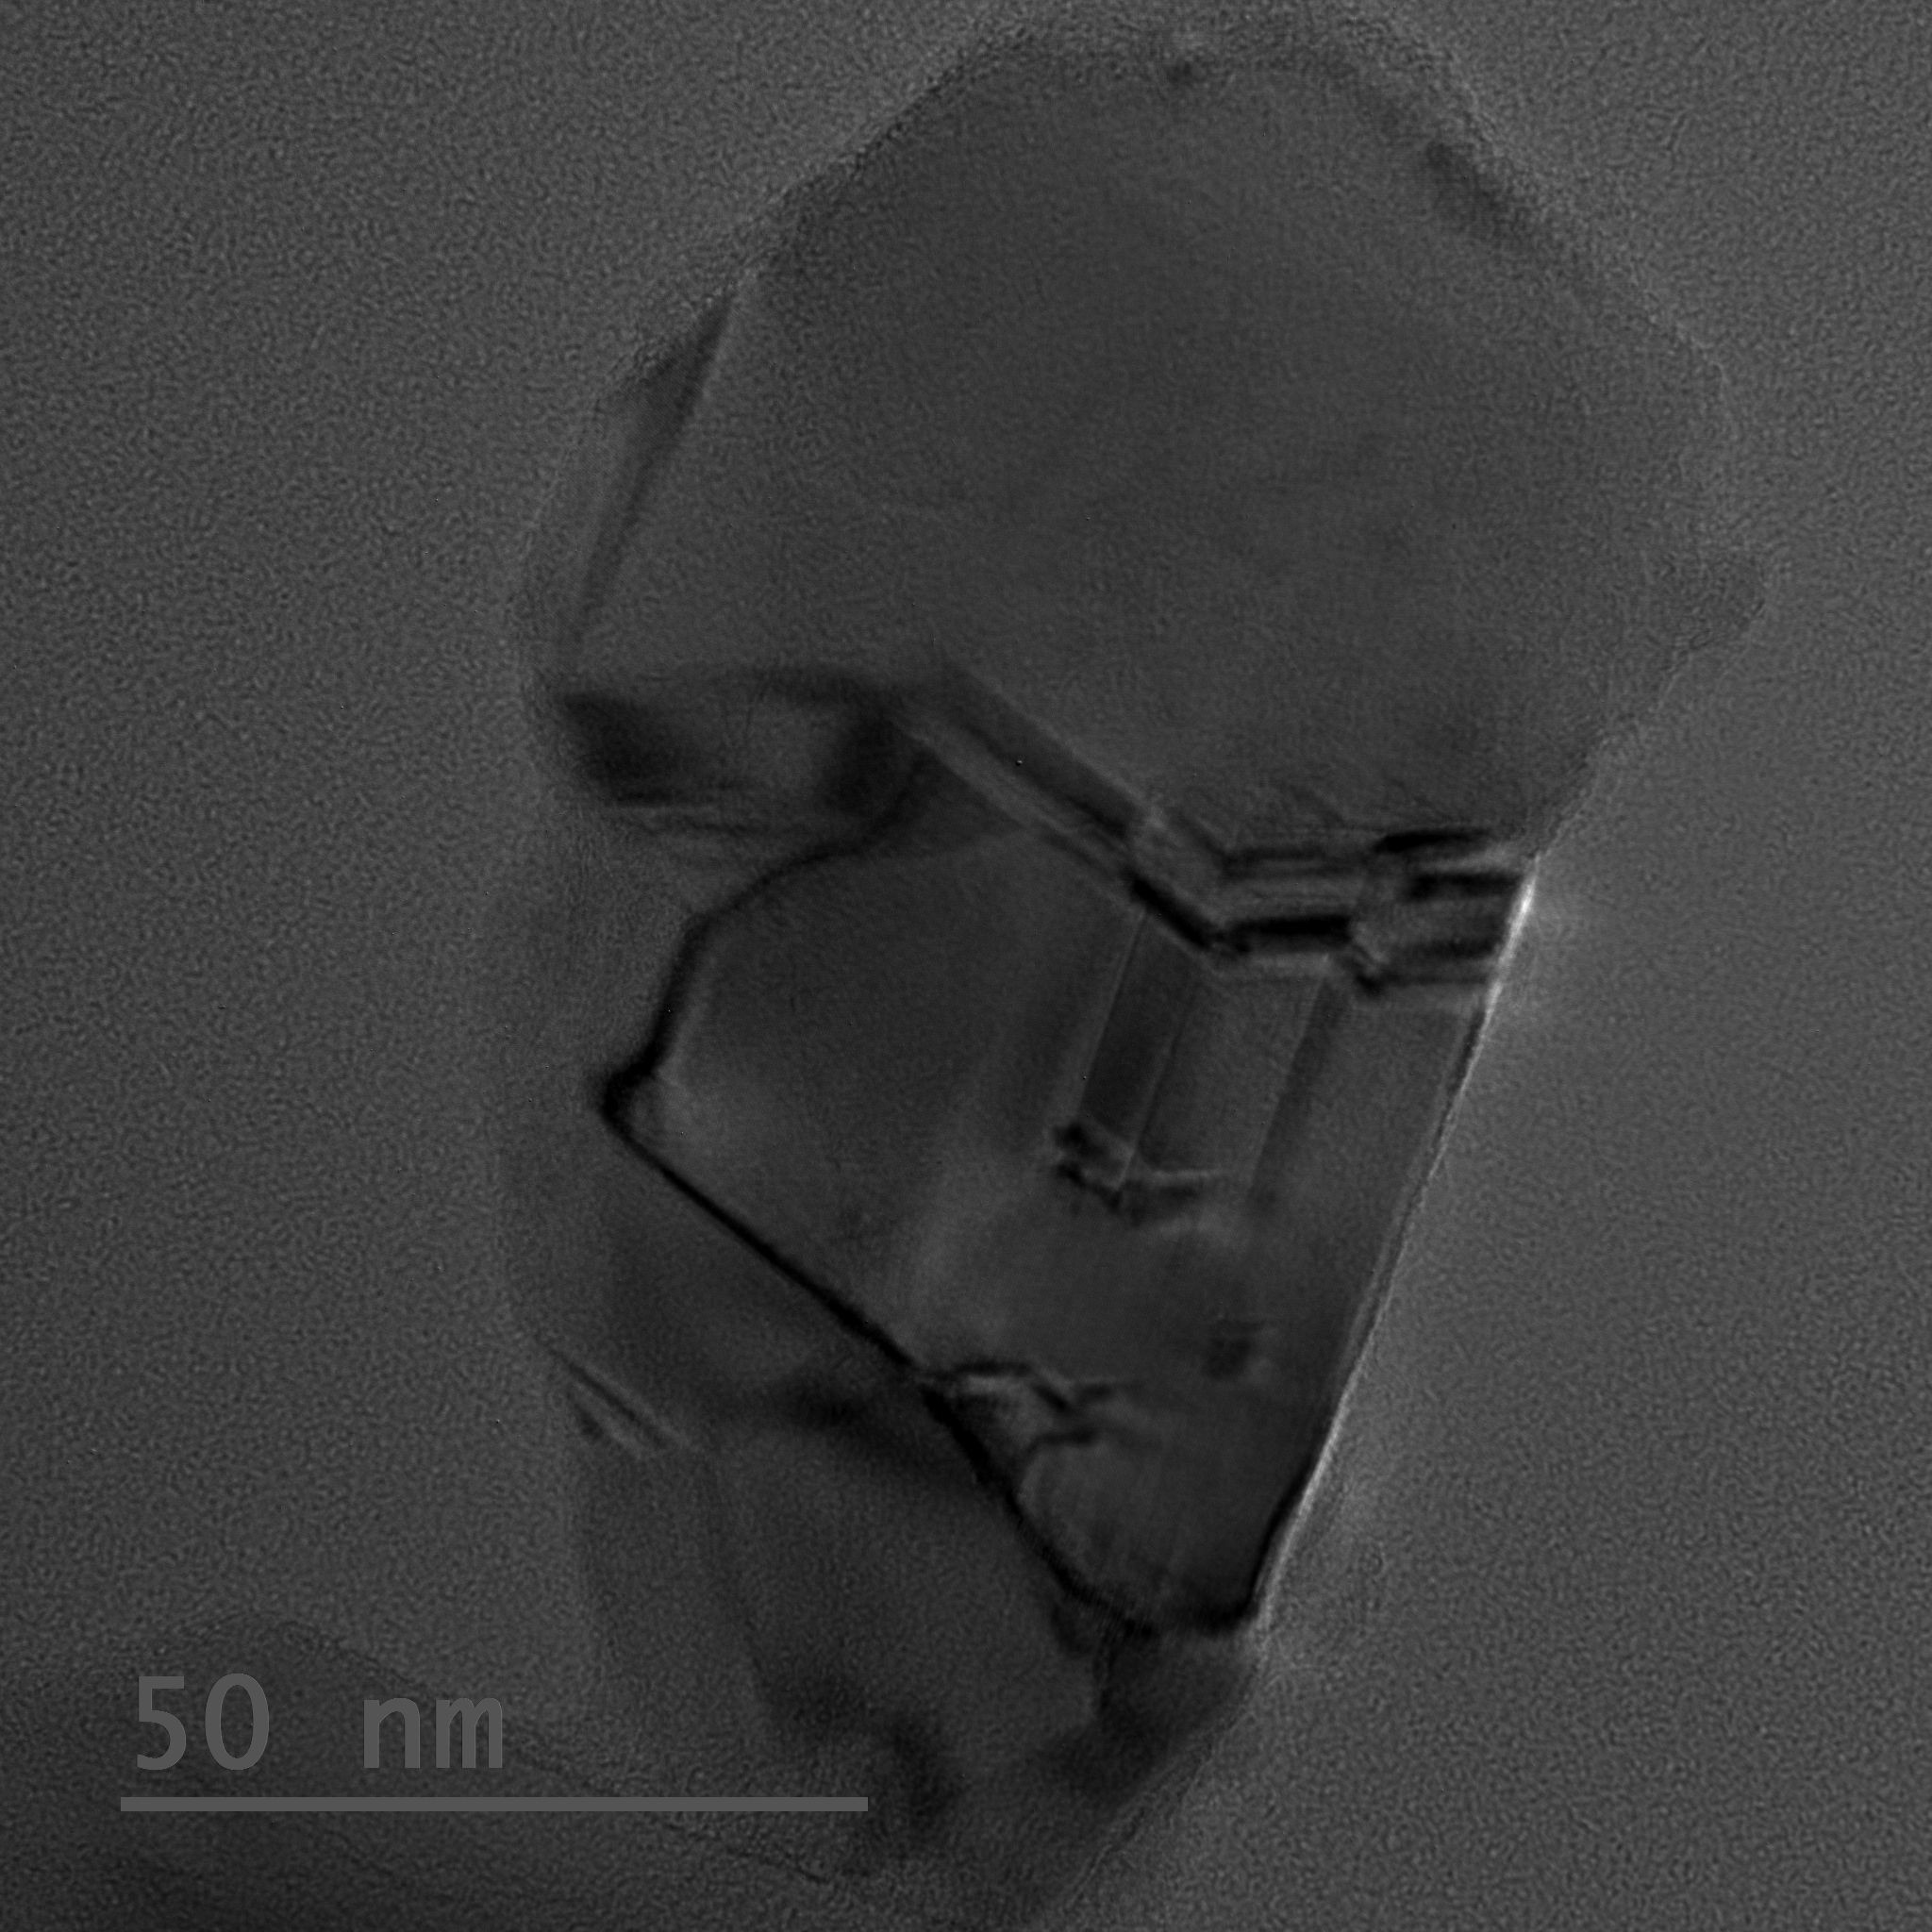
\includegraphics[trim = 0 0 0 0,  clip= true, height=5cm]{./pics/AM060-II-k4-2.jpg}}
			\caption{}\label{subfig::tem}
			% \caption{TEM picture of a \SI{100}{\nano\meter} diamond crystal.}
		\end{subfigure}
		\caption{Pictures of the milled \nds (sample \insituH). (a) SEM picture showing the distribution of the \nd crystals on the substrate. (b) TEM picture of a \nd particle.}
		\label{fig::semtem}
	\end{figure}



	\begin{table}[tp]
		\centering
		\caption{Overview of the investigated \nd samples. The columns indicate sample names, the mean diameter of the \nds, the \siv incorporation method, and the post-processing treatment(s) of the samples.} \label{tab::samplenames}
			\begin{tabular}{llll}
			\toprule
			Sample name & Diameter & Siv incorporation & post-processing \\
			\midrule
			\insituF & \SI{50}{nm} & \textit{in-situ} & \begin{tabular}[c]{@{}l@{}}series of individual samples with\\combinations of annealing and oxidation\end{tabular}\\ \hline
			\insituS & \SI{70}{nm} & \textit{in-situ} & \begin{tabular}[c]{@{}l@{}}series of individual samples with\\combinations of annealing and oxidation\end{tabular}\\ \hline
			\insituSn & \SI{70}{nm} & \textit{in-situ} &  \begin{tabular}[c]{@{}l@{}}no post-processing \\ subset of \insituS \end{tabular}\\ \hline
			\insituSo & \SI{70}{nm} & \textit{in-situ} & \begin{tabular}[c]{@{}l@{}}oxidized in air at \SI{450}{\celsius} \\ subset of \insituS \end{tabular}\\ \hline
			\insituH & \SI{100}{nm} & \textit{in-situ} & \begin{tabular}[c]{@{}l@{}}series of individual samples with\\combinations of annealing and oxidation\end{tabular}\\ \hline
			\insituHao & \SI{100}{nm} & \textit{in-situ} & \begin{tabular}[c]{@{}l@{}}annealed in vacuum at \SI{900}{\celsius}, \\ consecutively oxidized in air at \SI{450}{\celsius} \\ subset of \insituH \end{tabular}\\ \hline
			\implantedTao & \SI{250}{nm} & implanted & \begin{tabular}[c]{@{}l@{}}annealed in vacuum at \SI{900}{\celsius}, \\ consecutively oxidized in air at \SI{450}{\celsius}\end{tabular}\\
			\bottomrule
			\end{tabular}
	\end{table}
